\begin{testproblem}
\begin{equation}
\min_{x\in\R^2}\ (x_1 - 4)^2 + (x_2 - 7)^2
\end{equation}
\begin{equation*}
\begin{split}
\nb -10 \leq x_i & \leq 10,\ i = 1,2 \\
\end{split}
\end{equation*}
\end{testproblem}

\begin{testproblem}
(Rosenbrock-Funktion, vgl. Beispiel 1.4.1 in \cite[S.~14]{alt})
\begin{equation}
\min_{x\in\R^2}\ 100 (x_2-x_1^2)^2+(1-x_1)^2 
\end{equation}
\begin{equation*}
\begin{split}
\nb -10 \leq x_i & \leq 10,\ i = 1,2 \\
\end{split}
\end{equation*}
\end{testproblem}

\begin{figure}[h]
  \centering
  \includegraphics[width=0.45\textwidth]{rosenbrock}
  \includegraphics[width=0.45\textwidth]{himmelblau}
  \caption{Rosenbrock- und Himmelblau-Funktion}
  \label{fig:rosenbrock_und_himmelblau}
\end{figure}

\begin{testproblem}
(Himmelblau-Funktion, vgl. Beispiel 1.4.2 in \cite[S.~14f]{alt})
\begin{equation}
\min_{x\in\R^2}\ (x_1^2+x_2-11)^2 + (x_1+x_2^2-7)^2 
\end{equation}
\begin{equation*}
\begin{split}
\nb -10 \leq x_i & \leq 10,\ i = 1,2 \\
\end{split}
\end{equation*}
\end{testproblem}

\begin{testproblem}
(Bazaraa-Shetty-Funktion, vgl. Beispiel 1.4.3 in \cite[S.~15f]{alt})
\begin{equation}
\min_{x\in\R^2}\ (x_1-2)^4+(x_1-2 x_2)^2 
\end{equation}
\begin{equation*}
\begin{split}
\nb -10 \leq x_i & \leq 10,\ i = 1,2 \\
\end{split}
\end{equation*}
\end{testproblem}

\begin{testproblem}
(Vgl. Beispiel 1.4.4 in \cite[S.~16]{alt})
\begin{equation}
\min_{x\in\R^2}\ (1.5-x_1 (1-x_2))^2+(2.25-x_1 (1-x_2^2))^2+(2.625-x_1 (1-x_2^3))^2 
\end{equation}
\begin{equation*}
\begin{split}
\nb -10 \leq x_i & \leq 10,\ i = 1,2 \\
\end{split}
\end{equation*}
\end{testproblem}

\begin{testproblem}
\begin{equation}
\min_{x\in\R^2}\ e^{\|x\|^2} 
\end{equation}
\begin{equation*}
\begin{split}
\nb -10 \leq x_i & \leq 10,\ i = 1,2 \\
\end{split}
\end{equation*}
\end{testproblem}

\begin{figure}[h]
  \centering
  \includegraphics[width=0.45\textwidth]{bazaraa-shetty}
  \includegraphics[width=0.45\textwidth]{exp-func}
  \caption{Bazaraa-Shetty- und Exponent-Funktion}
  \label{fig:bazaraa_shetty_und_exp_funktion}
\end{figure}

\begin{testproblem}
\begin{equation}
\begin{split}
  \min_{x\in\R^4}\ & 100(x_2-x_1^2)^2 + (1-x_1)^2 + 90(x_4-x_3^2)^2 + (1-x_3)^2\\
    & + 10.1((x_2-1)^2 + (x_4-1)^2) + 19.8(x_2-1)(x_4-1)
\end{split}
\end{equation}
\begin{equation*}
\begin{split}
\nb -10 \leq x_i & \leq 10,\ i = 1,\ldots,4 \\
\end{split}
\end{equation*}
\end{testproblem}

\begin{testproblem}
\begin{equation}
\min_{x\in\R^3}\ (x_1 - 4)^2 + (x_2 - 2)^2 + (x_3 - 7)^2
\end{equation}
\begin{equation*}
\begin{split}
\nb 5 \leq x_i & \leq 10,\ i = 1,2,3 \\
\end{split}
\end{equation*}
\end{testproblem}

\begin{testproblem}
\begin{equation}
\min_{x\in\R^2}\ 100 (x_2-x_1^2)^2+(1-x_1)^2 
\end{equation}
\begin{equation*}
\begin{split}
\nb -10 \leq x_1 & \leq 10 \\
1.5 \leq x_2 & \leq 10 \\
\end{split}
\end{equation*}
\end{testproblem}

\begin{testproblem}
\begin{equation}
\min_{x\in\R^2}\ (x_1^2+x_2-11)^2 + (x_1+x_2^2-7)^2 
\end{equation}
\begin{equation*}
\begin{split}
\nb -10 \leq x_1 & \leq 10 \\
5 \leq x_2 & \leq 10 \\
\end{split}
\end{equation*}
\end{testproblem}

\begin{testproblem}
\begin{equation}
\min_{x\in\R^2}\ (x_1-2)^4+(x_1-2 x_2)^2 
\end{equation}
\begin{equation*}
\begin{split}
\nb 4 \leq x_1 & \leq 10 \\
-10 \leq x_2 & \leq 10 \\
\end{split}
\end{equation*}
\end{testproblem}

\begin{testproblem}
\begin{equation}
\min_{x\in\R^2}\ (1.5-x_1 (1-x_2))^2+(2.25-x_1 (1-x_2^2))^2+(2.625-x_1 (1-x_2^3))^2 
\end{equation}
\begin{equation*}
\begin{split}
\nb 3 \leq x_1 & \leq 10 \\
-10 \leq x_2 & \leq 10 \\
\end{split}
\end{equation*}
\end{testproblem}

\begin{testproblem}
\begin{equation}
\min_{x\in\R^3}\ e^{\|x\|^2} 
\end{equation}
\begin{equation*}
\begin{split}
\nb 0.5 \leq x_1 & \leq 10 \\
1 \leq x_i & \leq 10,\ i = 2,3 \\
\end{split}
\end{equation*}
\end{testproblem}

\begin{testproblem}
\begin{equation}
\begin{split}
  \min_{x\in\R^4}\ & 100(x_2-x_1^2)^2 + (1-x_1)^2 + 90(x_4-x_3^2)^2 + (1-x_3)^2\\
    & + 10.1((x_2-1)^2 + (x_4-1)^2) + 19.8(x_2-1)(x_4-1)
\end{split}
\end{equation}
\begin{equation*}
\begin{split}
\nb 2 \leq x_1 & \leq 10 \\
-10 \leq x_i & \leq 10,\ i = 2,3,4 \\
\end{split}
\end{equation*}
\end{testproblem}

\begin{testproblem}
\label{test_prob:lin_regres}
Lineare Regression (Vgl. Beispiel~\ref{example:lineare_regression})
\begin{equation}
\min_{x\in\R^2}\ \sum_{i=1}^{10} (x_1 \xi_i + x_2 - \eta_i)^2
\end{equation}
\begin{equation*}
\begin{split}
\nb -10 \leq x_i & \leq 10,\ i = 1,2 \\
\end{split}
\end{equation*}
Die Messwerte $(\xi_i,\eta_i), i = 1,\ldots,10,$
sind in der Tabelle~\ref{tbl:messwerte_lin_regres}
zu finden.
\end{testproblem}

\begin{table}[h]
\centering
\begin{tabular*}{0.8\linewidth}{@{\extracolsep{\fill}}c|cccccccccc}
  $\xi_i$ & 1 & 2 & 3 & 4 & 5 & 6 & 7 & 8 & 9 & 10 \\
  \midrule
  $\eta_i$ & $-0.5$ & $-2$ & $-3$ & $-3$ & $-2.5$
    & $-2$ & $-1$ & 1 & 3 & $5.5$ \\
\end{tabular*}
\caption{Messwerte f�r Testprobleme~\ref{test_prob:lin_regres}
und~\ref{test_prob:nichtlin_regres_quad}}
\label{tbl:messwerte_lin_regres}
\end{table}

\begin{testproblem}
\label{test_prob:nichtlin_regres_quad}
Nichtlineare Regression mit dem funktionalen
Zusammenhang~\eqref{eq:nichtlin_regres_quad_zusammenhang}
(Vgl. Beispiel~\ref{example:nichtlineare_regression})
\begin{equation}
\min_{x\in\R^3}\ \sum_{i=1}^{10} (x_1 (\xi_i -x_2)^2 + x_3 - \eta_i)^2
\end{equation}
\begin{equation*}
\begin{split}
\nb -10 \leq x_i & \leq 20,\ i = 1,2,3 \\
\end{split}
\end{equation*}
Die Messwerte
in der Tabelle~\ref{tbl:messwerte_lin_regres}
sind zu benutzen.
\end{testproblem}

\begin{figure}[h]
\centering
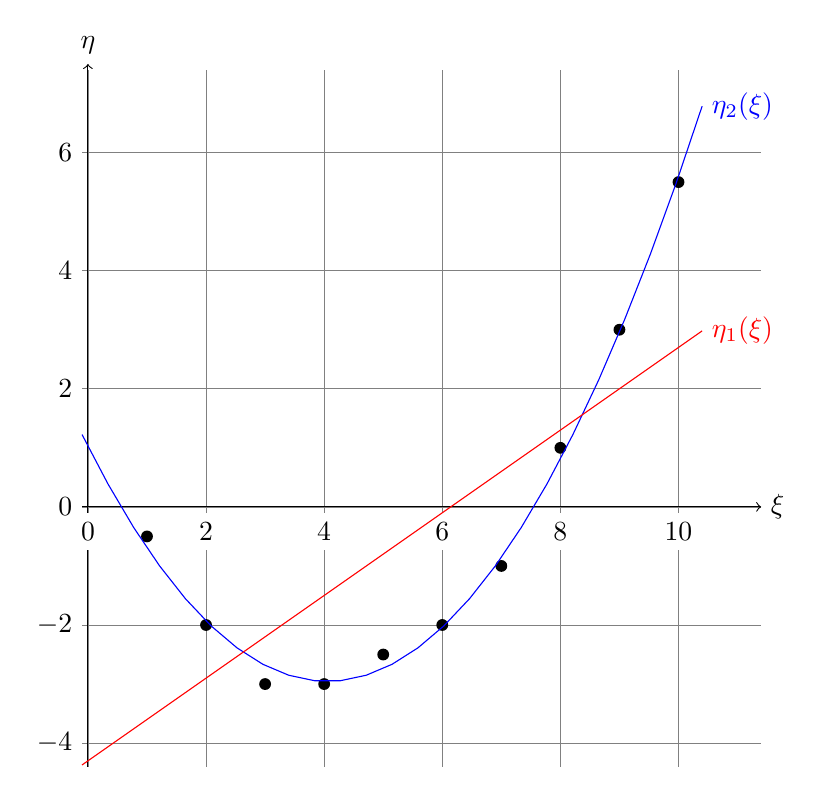
\begin{tikzpicture}[domain=-0.1:10.4,scale=0.75]
  \draw[very thin,color=gray,step=2] (-0.1,-4.4) grid (11.4,7.4);
  \draw[->] (-0.1,0) -- (11.4,0) node[right] {$\xi$};
  \draw[->] (0,-4.4) -- (0,7.5) node[above] {$\eta$};
  %\draw (-0.1,0.2) node [below left,fill=white] {0};
  \foreach \x in {0,2,4,...,10}
    \draw (\x,-0.1) node[below,fill=white] {$\x$};
  \foreach \y in {-4,-2,...,6}
    \draw (-0.1,\y) node[left] {$\y$};
  \foreach \x/\y in
    {1/-0.5, 2/-2, 3/-3, 4/-3, 5/-2.5, 6/-2, 7/-1, 8/1, 9/3, 10/5.5}
    \fill (\x,\y) circle(0.1);
  \draw[color=blue] plot (\x,{0.242*(\x-4.056)^2-2.955})
    node[right] {$\eta_2(\xi)$};
  \draw[color=red] plot (\x,{0.7*\x-4.3})
    node[right] {$\eta_1(\xi)$};
\end{tikzpicture}
\caption{L�sungen der Testprobleme~\ref{test_prob:lin_regres}
und~\ref{test_prob:nichtlin_regres_quad}}
\end{figure}

\begin{testproblem}
\label{test_prob:nichtlin_regres_exp}
Nichtlineare Regression mit dem funktionalen
Zusammenhang~\eqref{eq:nichtlin_regres_exp_zusammenhang}
(Vgl. Beispiel~\ref{example:nichtlineare_regression})
\begin{equation}
\min_{x\in\R^2}\ \sum_{i=1}^{10} (x_1 e^{\xi x_2} - \eta_i)^2
\end{equation}
\begin{equation*}
\begin{split}
\nb -10 \leq x_i & \leq 10,\ i = 1,2 \\
\end{split}
\end{equation*}
Die Messwerte $(\xi_i,\eta_i), i = 1,\ldots,10,$
sind in der Tabelle~\ref{tbl:messwerte_nichtlin_regres}
gegeben.
\end{testproblem}

\begin{table}[h]
\centering
\begin{tabular*}{0.8\linewidth}{@{\extracolsep{\fill}}c|cccccccccc}
  $\xi_i$ & 1 & 2 & 3 & 4 & 5 & 6 & 7 & 8 & 9 & 10 \\
  \midrule
  $\eta_i$ & 1 & 1.1 & 1.2 & 1.35 & 1.55
    & 1.75 & 2.5 & 3 & 3.7 & 4.5 \\
\end{tabular*}
\caption{Messwerte f�r Testproblem~\ref{test_prob:nichtlin_regres_exp}}
\label{tbl:messwerte_nichtlin_regres}
\end{table}
